\documentclass[11pt,a4paper]{article}

\usepackage[margin=2.6cm]{geometry}
\usepackage{amsmath,amssymb}
\usepackage{booktabs}
\usepackage{tikz}
\usepackage{xcolor}
\usepackage[colorlinks=true,linkcolor=black,citecolor=black]{hyperref}

\newcommand{\Stilde}{\widetilde{S}}
\newcommand{\Sth}{S_\theta}
\newcommand{\tr}{\operatorname{tr}}

\title{\bf The $\Gamma$ gap under disorder:\\ why a vanishing minimum is not a closing gap}
\author{}
\date{\today}

\begin{document}
\maketitle

\begin{abstract}
\noindent
In the disorder scan of the $Z_2$ marker, the quantity we plot as
``$\Delta_\Gamma$'' collapses as the disorder strength $W$ grows and does not
recover. This looks paradoxical: the Anderson disorder term is proportional to
the identity in the internal space, so it commutes with \emph{any} choice of
spin operator, and the spin structure ought to survive untouched. This note
shows that the paradox is an artefact of \emph{how the gap is defined}.
$\Delta_\Gamma$ is a \emph{minimum} over all $4L^2$ eigenvalues, and a minimum
over many samples is not a property of the bulk: it is an extreme-value
statistic. The bulk is in fact perfectly healthy --- the median eigenvalue
modulus is $0.992$ --- while the minimum is set by a handful of rare,
spatially localised resonances whose number grows linearly with system size.
The practical conclusion is that $\Delta_\Gamma$ should be reported as a
quantile rather than a minimum. The marker itself is shown to remain
well defined throughout.
\end{abstract}

\section{What the construction is supposed to do}

The one-parameter family of onsite ``spin'' operators is
\begin{equation}
  \Sth \;=\; \cos\theta \,\bigl(\tau_z\otimes\sigma_z\bigr)
           \;+\; \sin\theta \,\bigl(\tau_y\otimes\sigma_0\bigr).
  \label{eq:Stheta}
\end{equation}
The two terms anticommute, because $\{\tau_z,\tau_y\}=0$ while
$\sigma_z$ and $\sigma_0$ commute, and each squares to the identity. Hence
\begin{equation}
  \Sth^{\,2} \;=\; \cos^2\theta + \sin^2\theta \;=\; \mathbb{I},
\end{equation}
so $\Sth$ has eigenvalues $\pm 1$, each twofold degenerate, for every $\theta$.

From the one-particle density matrix $\rho = P$ (the projector onto the filled
bands, $P^2=P$) we build
\begin{equation}
  \Stilde \;=\; \rho\, \Sth + \Sth \rho - \Sth .
  \label{eq:Stilde}
\end{equation}
Writing $Q=\mathbb{I}-P$ for the projector onto the empty bands, a one-line
computation gives the form that makes the meaning transparent:
\begin{align}
  P\Sth P - Q\Sth Q
  &= P\Sth P - (\mathbb{I}-P)\Sth(\mathbb{I}-P) \nonumber\\
  &= P\Sth P - \Sth + \Sth P + P \Sth - P \Sth P \nonumber\\
  &= P\Sth + \Sth P - \Sth \;=\; \Stilde .
  \label{eq:PSPminusQSQ}
\end{align}
So $\Stilde$ acts as $+P\Sth P$ on the occupied subspace and as $-Q\Sth Q$ on
the empty one. Its spectrum is the spin content of the filled bands, with a
sign that separates the two sectors.

\paragraph{The ideal spectrum.} If $[\,H,\Sth\,]=0$ then $P$ and $\Sth$ can be
diagonalised together, every occupied state carries a sharp spin label
$\pm1$, and the spectrum of $\Stilde$ consists of two spikes:

\begin{center}
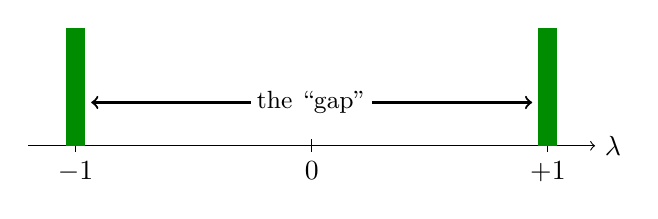
\begin{tikzpicture}[scale=1.0]
  \draw[->] (-3.6,0) -- (3.6,0) node[right] {$\lambda$};
  \foreach \x/\l in {-3/$-1$, 0/$0$, 3/$+1$}
    \draw (\x,0.08) -- (\x,-0.08) node[below] {\l};
  \fill[green!55!black] (-3.12,0) rectangle (-2.88,1.5);
  \fill[green!55!black] (2.88,0) rectangle (3.12,1.5);
  \draw[<->, thick] (-2.8,0.55) -- (2.8,0.55)
    node[midway,fill=white,inner sep=2pt] {\small the ``gap''};
\end{tikzpicture}
\end{center}

\noindent
The number we call $\Delta_\Gamma$ is the distance from $0$ to the nearest
eigenvalue,
\begin{equation}
  \Delta_\Gamma \;=\; \min_{n} \, |\lambda_n| ,
  \qquad n = 1,\dots,4L^2 .
  \label{eq:gapdef}
\end{equation}
Its purpose is to certify that the sign flattening
$\Stilde \mapsto \operatorname{sign}(\Stilde)$ is meaningful: if some
$\lambda_n$ sat exactly at zero, $\operatorname{sign}(0)=0$, we would have
$\Stilde^2\neq\mathbb{I}$, and the marker built on it would be meaningless.

\section{The puzzle}

The onsite part of the Hamiltonian is
\begin{equation}
  H_{\rm onsite} \;=\; M\,(\tau_z\otimes\sigma_0) \;+\; V_i\,\mathbb{I}_4 ,
  \qquad V_i \sim \mathcal{U}\!\left(-\tfrac{W}{2},\tfrac{W}{2}\right).
\end{equation}
The disorder enters as $V_i \mathbb{I}_4$ --- proportional to the identity in
the internal space. It therefore commutes with $\Sth$ for \emph{every}
$\theta$. As $W$ grows this term dominates $H$, the eigenstates localise, and
the naive expectation is unambiguous: the spin structure should become
\emph{better} defined, not worse, and $\Delta_\Gamma \to 1$.

What we observe instead is that $\Delta_\Gamma$ collapses around $W\approx10$
and stays small out to the largest $W$ we scan. Something has to give.

\paragraph{A tempting but wrong diagnosis.} One might check
$\lVert[H,\Sth]\rVert / \lVert H\rVert$ and find that it does decrease with
$W$ (from $0.87$ at $W=0$ to $0.11$ at $W=120$), apparently confirming the
intuition. But this ratio is misleading: the non-commuting part of $H$ (the
hoppings, and $M\tau_z$ against the $\tau_y$ component of $\Sth$) is
$W$-independent, while $\lVert H\rVert$ grows like $W$. The ratio shrinks for
trivial reasons. What decides whether $P$ and $\Sth$ can be diagonalised
together is not the size of $[H,\Sth]$ relative to $\lVert H\rVert$, but its
size relative to the \emph{level spacing between the states it connects}.
That distinction is the whole story, as we now show.

\section{The bulk is perfectly healthy}

Fix $W=30$ and look at the full distribution of $|\lambda_n|$, averaged over
$16$ disorder realisations, as the system size grows:

\begin{center}
\begin{tabular}{@{}rrrrrrr@{}}
\toprule
$L$ & states & $\min|\lambda|$ ($=\Delta_\Gamma$) & 1st pct & 5th pct & median & \# with $|\lambda|<0.5$ \\
\midrule
 6 & 144 & 0.449 & 0.449 & 0.678 & 0.9918 &  2.8 \\
 8 & 256 & 0.357 & 0.357 & 0.701 & 0.9923 &  5.5 \\
10 & 400 & 0.326 & 0.491 & 0.710 & 0.9924 &  5.8 \\
12 & 576 & 0.319 & 0.437 & 0.700 & 0.9925 &  9.8 \\
14 & 784 & 0.313 & 0.469 & 0.702 & 0.9926 & 12.2 \\
\bottomrule
\end{tabular}
\end{center}

\noindent
Read the columns from right to left and the picture assembles itself:

\begin{itemize}
  \item The \textbf{median} is $0.992$ at every size. More than $98\%$ of
        states sit essentially exactly at $\pm1$, which is precisely the
        Anderson-type behaviour we expected. The bulk spin structure is intact.
  \item Every \textbf{quantile} is flat in $L$. The $5$th percentile is
        $0.70$ whether the system has $144$ or $784$ states.
  \item Only the \textbf{minimum} moves, and it moves \emph{downwards with
        system size} at fixed disorder.
  \item The \textbf{number} of spoiled states grows roughly in proportion to
        the number of sites ($36\to196$ sites, $2.8\to12.2$ states), so their
        \emph{fraction} is constant.
\end{itemize}

\noindent
Nothing here depends on $W$ at all --- the disorder is fixed. The apparent
degradation is entirely a function of how many states we sampled.

\section{Minimum versus typical: the heart of the matter}

Suppose each $|\lambda_n|$ is a draw from a distribution overwhelmingly
concentrated near $1$, with a thin tail reaching down towards $0$. The
definition \eqref{eq:gapdef} asks for the \emph{worst single draw} out of
$4L^2$. The more draws you take, the further into the tail you reach --- even
though the distribution never changed.

\begin{quote}
\emph{An analogy.} Measure everyone's height in a village and in a city. The
distributions are identical: same mean, same percentiles. But ``how short is
the shortest person?'' returns a much smaller number in the city, purely
because more people were sampled. Nobody got shorter.
\end{quote}

\noindent
It is worth separating three quantities that the single symbol
$\Delta_\Gamma$ silently conflates:
\begin{center}
\begin{tabular}{@{}lll@{}}
\toprule
quantity & scaling & interpretation \\
\midrule
\emph{fraction} of spoiled states & $\sim t/W$ & physical, size independent, falls with disorder \\
\emph{number} of spoiled states   & $\sim N t/W$ & grows with the system \\
\emph{the worst one} ($\Delta_\Gamma$) & --- & extreme-value statistic \\
\bottomrule
\end{tabular}
\end{center}
Only the first is a property of the disordered phase. The intuition about the
Anderson theorem applies to it, and --- as the table in the previous section
shows --- that intuition is correct. It simply is not what we plotted.

\section{Where the spoiled states come from}

The mechanism is a rare-resonance effect, and it survives however weak the
symmetry-breaking coupling is.

Take two nearby sites whose random onsite energies happen to come out almost
equal, $|V_i-V_j| = \Delta E$, coupled by a hopping matrix element $t$.
Two-level degenerate perturbation theory gives a mixing angle
\begin{equation}
  \tan 2\alpha \;=\; \frac{2t}{\Delta E} ,
\end{equation}
so that when $\Delta E \ll t$ the eigenstates are \emph{maximal} $50/50$
superpositions --- no matter how small $t$ is. An arbitrarily weak coupling
completely scrambles an accidentally degenerate pair.

Crucially, the hopping matrices in this model,
\begin{equation}
  A\,\tau_z\sigma_0
  - \mathrm{i}A\,\tau_x(\cos\phi\,\sigma_x + \sin\phi\,\sigma_y)
  - \mathrm{i}\lambda_R\,\tau_0(\sin\phi\,\sigma_x - \cos\phi\,\sigma_y)
  - \mathrm{i}\lambda_D\,\tau_0(\cos\phi\,\sigma_x - \sin\phi\,\sigma_y),
\end{equation}
do \emph{not} commute with $\Sth$. So a resonant pair produces an eigenstate
with no definite spin character, i.e.\ $\lambda \approx 0$.

\paragraph{How often?} We need $|V_i - V_j| \lesssim t$ with the $V$'s spread
over a range $W$, giving a probability $\sim t/W$ per pair. This is small, and
it \emph{decreases} with disorder exactly as intuition demands. But there are
$\mathcal{O}(N)$ pairs, so the expected number of spoiled states is
\begin{equation}
  n_{\rm spoiled} \;\sim\; N\,\frac{t}{W} .
  \label{eq:counting}
\end{equation}
The minimum over the whole system only recovers once $n_{\rm spoiled}\lesssim1$,
that is
\begin{equation}
  \boxed{\;W \;\gtrsim\; N\,t\;}
\end{equation}
which for $L=14$ ($N=196$) means $W\gtrsim200$. Our scans stop at $W=30$. This
is why the recovery is never seen in the plotted window --- and it explains the
measured numbers quantitatively: at $W=60$ and $W=120$ the gap does climb back,
to $0.57$ and $0.59$, but slowly.

\paragraph{The states are localised.} Direct confirmation: the eigenvector
attached to $\min|\lambda|$ has an inverse participation ratio of
$0.14$--$0.49$ at $W=30$--$60$, with weight on only $3$--$15$ sites out of
hundreds. These are not bulk excitations; they are isolated accidents.

\paragraph{A control.} Setting $M=0$ makes the onsite term exactly
$V_i\mathbb{I}_4$, which commutes with everything, removing the intra-site
$\tau_z$-doublet channel. It helps, but only partially
($0.284 \to 0.343$ at $W=30$; $0.529\to0.672$ at $W=60$, at $L=12$), confirming
that inter-site resonances --- not the $M\tau_z$ term --- dominate.

\section{Two effects are superimposed}

The measured curve is the sum of one real effect and one artefact.

\begin{enumerate}
  \item \textbf{The dip near $W\approx10$--$15$ is genuine.} It coincides with
        the marker going from $-1$ to $0$: this is the topological transition,
        where the mobility gap closes and states genuinely delocalise and
        scramble. This feature should be kept and reported.
  \item \textbf{The failure to recover afterwards is the artefact.} Deep in
        the trivial phase the minimum should climb back, and by
        \eqref{eq:counting} it needs $W \gtrsim Nt$ before it does. Within the
        plotted window one sees only the very beginning of the recovery, so
        the curve reads as permanently closed.
\end{enumerate}

\paragraph{A ceiling that is not $1$.} Even in the ideal limit the gap does not
reach unity for $\theta \neq 0$. On a site where only the $\tau_z=+1$ doublet
is filled, $P$ projects onto that subspace, and since $\tau_y$ is purely
off-diagonal in the $\tau_z$ basis,
\begin{equation}
  \langle \tau_z=+1 | \Sth | \tau_z = +1\rangle \;=\; \cos\theta\;\sigma_z
  \quad\Longrightarrow\quad
  \lambda = \pm\cos\theta .
\end{equation}
So the attainable ceiling is $\cos\theta_k = 0.8817$ for our working angle.
This is confirmed independently by the clean mass scan ($W=0.25$), where
$\Delta_\Gamma$ sits on a flat plateau at exactly $0.88$ away from the
transition.

\paragraph{A related caveat on $\theta$.} The analytic angle $\theta_k$ is
derived for the \emph{clean} lattice and is used unchanged across the whole
disorder scan. At strong disorder the optimum drifts towards $\theta=0$, where
$\Sth = \tau_z\sigma_z$ commutes with both $M\tau_z$ and $V_i\mathbb{I}_4$. At
$W=30$ the numerically optimal angle is $\theta=0$, not $\theta_k=0.49$. This
is a genuine but secondary effect: near the transition the gap is small at
\emph{every} $\theta$, so a better angle does not rescue it.

\section{Is the marker still well defined?}

This is the question that matters, and it needs care, because ``the gap is
small'' and ``the construction is broken'' are not the same statement.

\begin{itemize}
  \item If $\lambda = 0$ \emph{exactly}, then $\operatorname{sign}(0)=0$,
        $\Stilde^2 \neq \mathbb{I}$, and the marker is meaningless. This is a
        hard failure.
  \item If $\lambda$ is small but nonzero, $\operatorname{sign}(\lambda)$
        returns $\pm1$ perfectly well, $\Stilde^2 = \mathbb{I}$ holds
        \emph{exactly}, and the marker is well defined. What is fragile is only
        \emph{which sector that particular state was assigned to}.
\end{itemize}

\noindent
Measured at $L=12$: the smallest $|\lambda|$ anywhere in the whole scan is
$0.025$, against a zero-mode tolerance of $10^{-8}$. Not one state comes within
$0.02$ of zero. The construction never fails.

For stability, we can deliberately reassign the ambiguous states to the
opposite sector and see how far the marker moves:

\begin{center}
\begin{tabular}{@{}rrrrr@{}}
\toprule
$W$ & $\min|\lambda|$ & marker & \# with $|\lambda|<0.1$ & $\delta$(marker) if flipped \\
\midrule
 5 & 0.737 & $-0.979$ & 0 & $0$ \\
10 & 0.090 & $-0.716$ & 4 & $+0.049$ \\
12 & 0.086 & $-0.595$ & 4 & $+0.084$ \\
14 & 0.037 & $-0.313$ & 4 & $+0.001$ \\
15 & 0.025 & $-0.198$ & 4 & $-0.009$ \\
20 & 0.075 & $-0.088$ & 4 & $+0.037$ \\
30 & 0.190 & $-0.009$ & 0 & $0$ \\
\bottomrule
\end{tabular}
\end{center}

\noindent
Away from the transition ($W=5$, $W=30$) there are no ambiguous states at all
and the marker is exactly unchanged. Near the transition a single Kramers
quartet is ambiguous, and flipping it shifts the marker by up to $0.084$ on a
scale of $[-1,0]$.

That residual sensitivity is not a defect. It is the standard \emph{mobility
gap} situation, familiar from the integer quantum Hall effect: one does not
need a spectral gap in $P\Sth P$, only that the states near $\lambda=0$ be
\emph{localised}. A localised state carries no Chern number, so moving it
between the two spin sectors leaves $C_\pm$ unchanged and the topology does
not notice. The measured inverse participation ratios confirm the states are
localised. And the surviving sensitivity sits exactly at $W\approx12$, the
critical point, where the invariant genuinely is not sharp and
sample-to-sample fluctuation \emph{is} the physics. A marker that showed no
sensitivity at criticality would be the suspicious result.

\section{What to report instead}

\begin{enumerate}
  \item \textbf{For the figure,} plot a \emph{quantile} of $|\lambda|$ (the
        $1$st or $5$th percentile) rather than the minimum. These are
        self-averaging, independent of system size, and genuinely measure how
        much spin structure survives.
  \item \textbf{As a diagnostic,} report the \emph{count} of states below a
        small threshold. This is $0$ away from the transition and $4$ near it,
        and it answers directly the question ``how many sector assignments
        were coin flips?''
  \item \textbf{Keep the minimum} for the one job it is right for: the
        numerical assertion that no eigenvalue sits at machine zero, which is
        what the existing \texttt{zero\_mode\_tol} warning uses it for.
\end{enumerate}

\noindent
The practical urgency is that the minimum drifts downwards with every increase
in system size at fixed disorder. In a finite-size scaling plot that drift will
read as physics when it is arithmetic.

\appendix
\section{Numerical details}

All data were produced with the amorphous lattice at $w=0.1$, $r=1.3$, closed
(periodic) boundaries, $A=1$, $\lambda_R=1$, $\lambda_D=0.5$, $M=-2$ unless
stated otherwise, and $\theta_k = 0.4914$ from
$\theta_k = \tfrac12[\arctan\frac{\lambda_R+\lambda_D}{A}
+ \arctan\frac{\min(0,\lambda_R-\lambda_D)}{A}]$.
The Hilbert space dimension is $D = 4L^2$. Quantile and count statistics are
averaged over $16$ disorder realisations; the $M=0$ control over $8$. The
inverse participation ratio is computed on site-resolved weights,
$\mathrm{IPR} = \sum_i \bigl(\sum_{\alpha}|v_{i\alpha}|^2\bigr)^2$, so that
$\mathrm{IPR}\sim1/N$ indicates an extended state and $\mathrm{IPR}=O(1)$ a
state on a few sites.

\end{document}
